\documentclass[twocolumn]{aastex62}

\newcommand{\vdag}{(v)^\dagger}
\newcommand\aastex{AAS\TeX}
\newcommand\latex{La\TeX}
\usepackage{amsmath}
\usepackage{physics}
\usepackage{hyperref}
\usepackage{natbib}
\usepackage[T1]{fontenc}
\usepackage[english]{babel}
\usepackage[utf8]{inputenc}

\begin{document}

\title{\Large Orbital Mechanics Simulations by Means of Numerical Methods}

\author{Håkon Tansem}

\author{Nils-Ole Stutzer}

\author{Bernhard Nornes Lotsberg}

\begin{abstract}

\end{abstract}

\section{Introduction} \label{sec:intro}
Celestial mechanics is a physical problem that has intreeged mankind since the
day of time. It has fascinated astronomers since night time observations done by
the antient greeks, through Galileo Galilei's studies of Jupiters moons in the
Renaissance, to todays detailed observations and simulations. At the present
date one can do detailed numerical simulations of the motion of planets and
other celestial objects, so as to predict their motion many centuries into the
future.

In this paper we will study how the celestial bodies in our Solar System
interact using two different numerical methods for solving the coupled
differential equations of motion discribing their movement. We will look at the
classical Forward Euler and the more advanced Velocity Verlet methods, and
compare them. In addition we will study different versions of the gravitational
force to see how it affects the planets orbit, and also we will see what happens
to the Earth's and Sun's motion if Jupiters mass is changes. Last we will study
Mercury's perihelion precession.

We will present theory and its implementation in the Method section. The results
of our study will be presented and discussed in the Results and Discussion
section respectively.


\section{Method} \label{sec:method}
\subsection{The Gravitational force and the Equations of Motion}\label{subsec:gravity}
The motion of celectial bodies in the solar system are governed by one single
force, being the gravitational force. In Newtonian physics this is written as
\begin{align}
    \vec{F} = -G\frac{Mm}{r^3}\vec{r},
\end{align}
where $F$ is the force between two masses $M$ and $m$ separated by a distance
$\vec{r}$ ($r = |\vec{r}|$) and $G$ is the gravitational constant. More
generally when having more than just two celectial bodies ($N$ bodies), the force on one of
them $m_i$ is simply the sum of the gravitational force from all the other
bodies $m_j$. Thus we have the total gravitational force 
\begin{align}
    \vec{F}_i = \sum_i^N \sum_{j\neq i}^N -G\frac{m_im_j}{|\vec{r}_j - \vec{r}_i|^3}(\vec{r}_j - \vec{r}_i) = m_i \vec{a}_i = m_i \ddot{\vec{r}}_i,
    \label{eq:newtonian_gravity}
\end{align}
where we used Newton's second law to find the acceleration. In this $N$-body problem
celectial bodies are interacing with each other, affecting each others motions.
When simulating our Solar System, it is often common to let the Sun be static at
the origin due to its mass being many orders of magnitude larger than that of
the planet, limiting its motion to a small wiggle. We will however include the
Suns motion in our simulations, as it reflects reality better than having it
static. 

When simulating the motions of the celectial bodies according to the force
(\ref{eq:newtonian_gravity}) it is convenient to chose a scaling more suited to
the scales of the Solar System. To find such a scaling we consider the
gravitational force between Earth and the Sun in a circular orbit. We then get 
\begin{align}
    F = G\frac{M_\oplus M_\odot}{r^2} = \frac{v^2}{r}M_\oplus,
\end{align}
using that gravity equals the centripetal force in a circular orbit. Since we
know that for a circualr orbit $v = \frac{2\pi r}{T}$, for an orbital periode $T
= 1\rm{yr}$, we get that the gravitational constant becomes
\begin{align}
    G = 4\pi^2 \frac{\rm{AU}^3}{\rm{yr}^2 M_\odot},
\end{align}
since the relative Sun-Earth distance in a circular orbit is $1\rm{AU}$. Thus we
use units solar masses $M_\odot$, astronomical units $\rm{AU}$ for distances and
years
$\rm{yr}$ for time, as they are far easier to handle. 

In order to solve the equations of motion we can write the second order ordinary
differentail equation (ODE) as a system of two coupled first order equations.
Further more as the equations are vector equations, we can write the coupled
system of equations for body $i$ component wise as 
\begin{align}
    v_x^i = \dv{x^i}{t} = \dot{x}^i \text{ and } a_x^i = \dv{v_x^i}{t} = \dot{v}_x^i,
    \label{eq:coupled_odes}
\end{align}
and similarly for the $y$ and $z$ components. Thus when simulation $N$ bodies in
three dimensions we would need $6N$ coupled differential equations. 



\subsection{discretization and Numerical Solvers}
When solving the system of $6N$ coupled ODEs numically we need to discretize the
equations. We do this by letting $x(t)\to x(t_i) = x_i$ where the time $t \to
t_i = a + ih$, with $t\in[a, b]$ and $i = 0, 1, 2, \ldots n-1$. Then $a\to t_0$
, $b\to t_n$ and the time step $h = \frac{b-a}{n}$ for $n$ time steps. Using this discretization the position in the next time step is
written as $x(t_i + h) = x_{i+1}$. 

From the taylor expansion 
\begin{align}
    x_{i+1} = x_i + h\dot{x}_i + \frac{h^2}{2}\ddot{x}_i + \mathcal{O}(h^3)
\end{align}
we can get Eulers Forward algorithm when only keeping first order terms.
This then becomes 
\begin{align}
    x_{i+1} = x_i + hv_x^i + \mathcal{O}(h^2),
\end{align}
inserting that $v_x^i = \dot{x}_i$. Similarly, the second coupled ODE can be
written
\begin{align}
    v_x^{i+1} = v_x^i + h  \dot{v}_x^i = v_x^i + h  a_x^i + \mathcal{O}(h^2).
\end{align} 
This algorithm is very simple and requires only a few floating point operations
(FLOPs) per time step, however, the traid-off is that it is quite
inacurate having an error term $\mathcal(O)(h^2)$.

Another numerical method more comonly used is the Velocity Verlet algoritm. It
has the advantage of being more accurate than the Forward Euler, having a
mathematical error term of $\mathcal{O}(h^3)$, in addition to requireing about
the same amont of FLOPs. Also it is taylored towards conserving the total
mechanical energy and angular momentum of a Hamiltonian system such as a
$N$-body system, because it is a symplectic integration scheme (KILDER). We can write the
two coupled ODEs as 
\begin{align}
    x_{i+1} &= x_i + hv_x^i + \frac{h^2}{2}a_x^i + \mathcal{O}(h^3)\\
    v_x^{i+1} &= v_x^i + \frac{h}{2}[a_x^{i+1} + a_x^i] + \mathcal{O}(h^3).
\end{align}
As oppose to the Forward Euler we see that the two equations in this scheme are
not independent of eachother. To solve for the velcity at the next time step one
needs the acceleration for the next time step as well. This acceleration is
found through the next position $x_{i+1}$. These two equations thus always have
to be solved together. Comparing the amount of FLOPs per time step, we find that
the Forward Euler algorithm has about 4 flops per step, while the Velocity
Verlet scheme has 7 if $h/2$ and $h^2/2$ are precalculated. This is remarcable,
as one can constuct a scheme with a supperior error conserving energy and
angular momentum with only a few FLOPs extra. The drawback is of course that one
has to compute an acceleration two times per step using the Velocity Verlet
scheme, which was not taken into account when counting the FLOPs as the FLOPs in
the acceleration are dependent on how many bodies are simulated.
As both schemes have similar amounts of FLOPs we expect them to perform
similarly in a timing of the algorithms.


\subsection{Testing the algorithms} \label{subsec:algo_test}
We know from classical mechanics that there are certain quantities that are
constant over time, the so-called constants of motion. In our case where we
consider a system of interacting in a conservative force potensial, the kinetic $K$,
potensial $V$ and total mechanical energy $E$ as well as the angular momentum $l$ are such
constants of motion. If we consider a Sun-Earth system in the plane of the
motion we get that Earth has a Lagranian 
\begin{align}
    L = K + V = \frac{1}{2}M_\oplus(\dot{r}^2 + r^2\dot{\phi}^2) + G\frac{M_\oplus M_\odot}{r},
\end{align}
for an angular velocity $dot{\phi}$. We see that since the Lagranian $L$ is
independent of the azimuth angle $\phi$ we get from Lagranges equation that 
\begin{align}
    \dv{t}\pdv{L}{\dot{\phi}} - \pdv{L}{\phi} = \dv{t}\pdv{L}{\dot{\phi}} = 0,
\end{align}
gives us that 
\begin{align}
    \implies l = \pdv{L}{\dot{\phi}} = m r^2 \dot{\phi} = \rm{constant}.
\end{align}
This is a constant of Noether's theorem, where all symetries of a system result
in a constant of motion (KILDE), such as the invatiance under an azimuth rotation in our
case. Furthermore, since there are no rigid-body constaints in our system that
are time-dependent the total energy of the system is given by the Hamiltonian $H
= E = K + V$. If we have a explicitly time-independent Lagrangian it follows
that the implicit time dependence of the Hamiltonian is given as 
\begin{align}
    \dv{H}{t} = \dv{E}{t} = \pdv{L}{t} = 0,
\end{align} 
which implies that the total energy of our system must be conserved (KILDER). In
the special case of a circular orbit the kinetic and potensial energies are also
conserved, because the constant distance $r$ to the center of mass (CM) gives a
constant potential energy and a constant orbital speed $v =
\sqrt{\frac{GM_\odot}{r}}$, i.e. a constant kinetic energy. 

To chenck whether our numerical schemes conserve the constants of motion we
simulate a Sun-Earth system over several years and plot the energies and angular
momentum against time. When doing this we must correct for the motion of the CM
as it is the angular momentum around the CM that is constant. The center of mass
is given by the position $\vec{R}_\mathrm{CM}$ and the velocity
$\vec{V}_\mathrm{CM}$ as 
\begin{align}
    \vec{R}_\mathrm{CM} &= \frac{1}{M_\mathrm{tot}}\sum_i^N m_i \vec{r}_i\\
    \vec{V}_\mathrm{CM} &= \frac{1}{M_\mathrm{tot}}\sum_i^N m_i \vec{v}_i
\end{align}
for the total mass $M_\mathrm{tot}$.

Also to research the stability of the two algorithms over
time we simulate several Sun-Earth systems using different time steps $h$ and
chenck how close to thir staring point thay get after one orbit. 

\subsection{Escape Velocity and Modifies Gravitational Force}
Next we will consider a Sun-Earth system where the Earth starts 1 AU from the
Sun.


\section{Results} \label{sec:results}
\begin{figure}
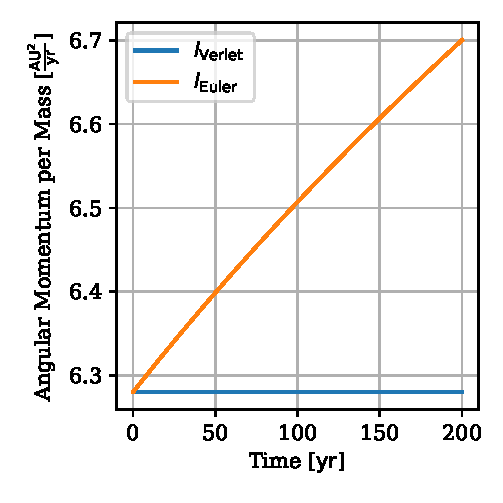
\includegraphics[scale=1]{Figures/taskb_angmom.pdf}
\caption{Angular momentum for Euler and Verlet.}
\label{fig:angmom}
\end{figure}


\begin{figure}
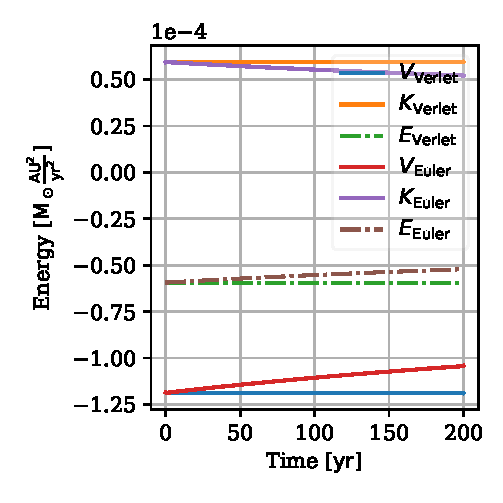
\includegraphics[scale=1]{Figures/taskb_energies.pdf}
\caption{Energies for Euler and Verlet}
\label{fig:energy}
\end{figure}

\begin{figure}
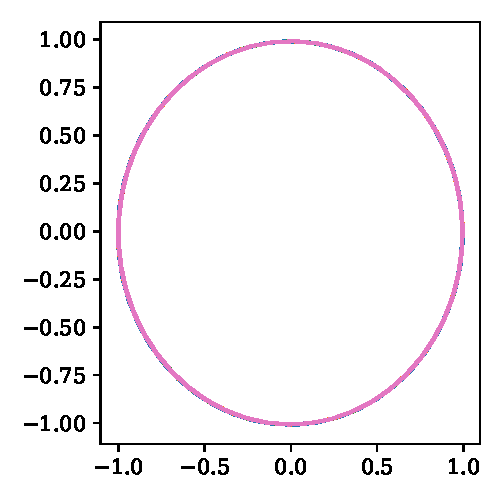
\includegraphics[scale=1]{Figures/taskb_trajectories.pdf}
\caption{Trajectory Sun and Earth}
\label{fig:traj}
\end{figure}

\begin{figure*}
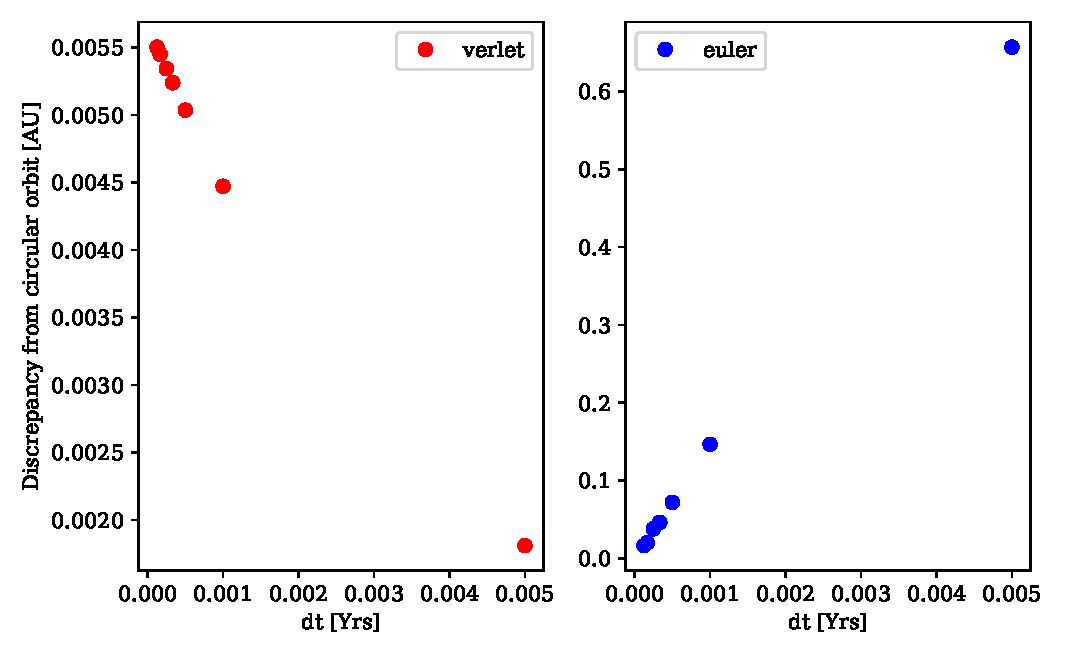
\includegraphics[scale=1]{Figures/taskb_errors.pdf}
\caption{Errors Euler and Verlet}
\label{fig:error}
\end{figure*}

\begin{figure}
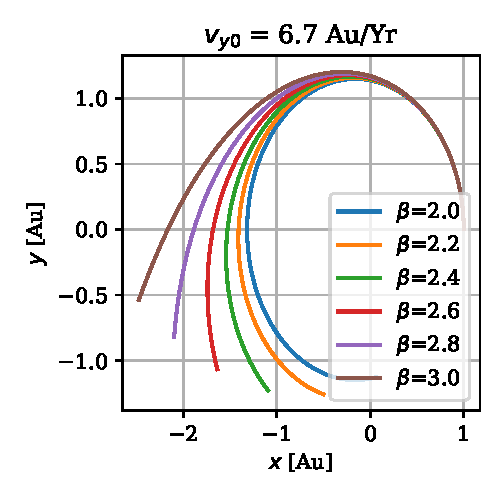
\includegraphics[scale=1]{Figures/beta.pdf}
\caption{Trajectory Earth Sun different $\beta$.}
\label{fig:beta}
\end{figure}

\begin{figure}
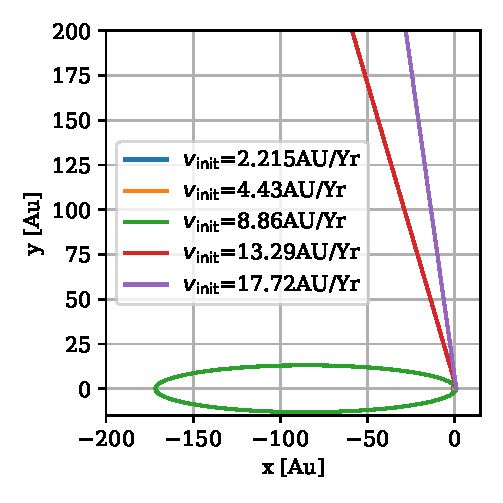
\includegraphics[scale=1]{Figures/espace.pdf}
\caption{Different velocities for Earth Sun system.}
\label{fig:escape}
\end{figure}

\begin{figure}
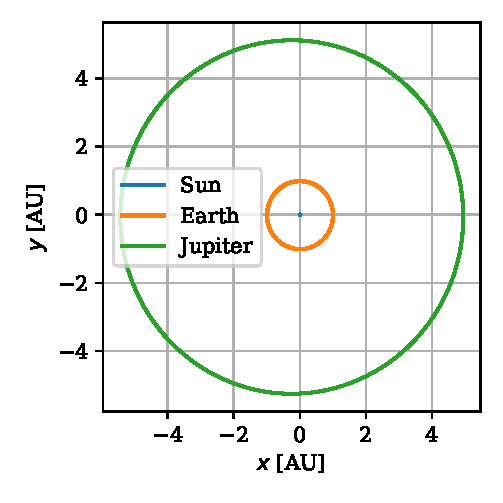
\includegraphics[scale=1]{Figures/jupiter.pdf}
\caption{Jupiter normal weight}
\label{fig:jupiter}
\end{figure}

\begin{figure}
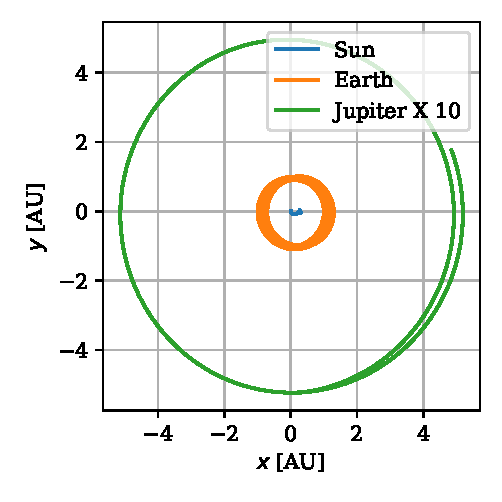
\includegraphics[scale=1]{Figures/jupiter10.pdf}
\caption{Jupiter ten times size}
\label{fig:jupiter10}
\end{figure}

\begin{figure}
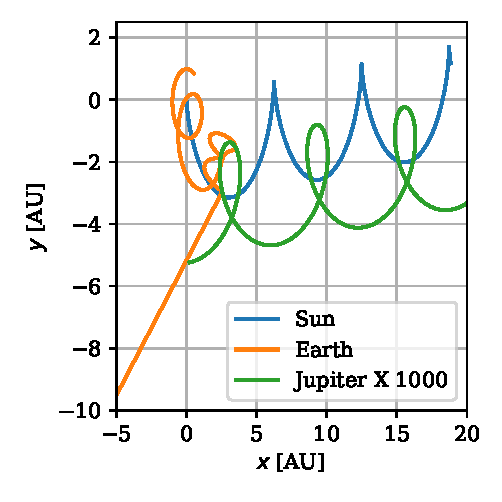
\includegraphics[scale=1]{Figures/jupiter1000.pdf}
\caption{Jupiter 1000 times size}
\label{fig:jupiter1000}
\end{figure}

\begin{figure*}
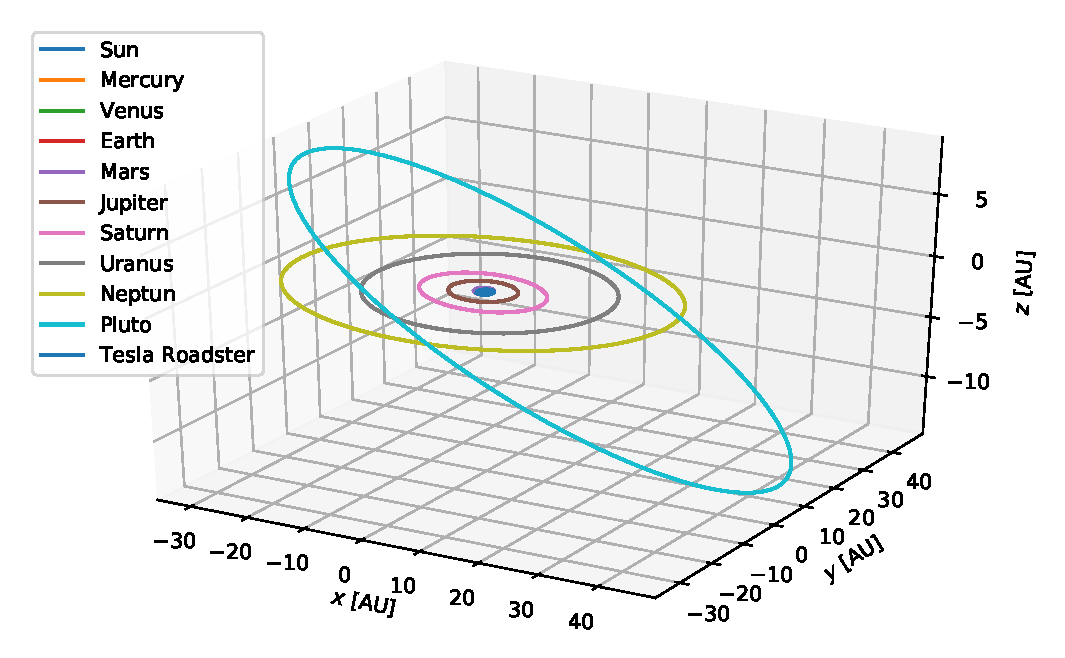
\includegraphics[scale=1]{Figures/OuterSolarSystem.pdf}
\caption{Full solar system}
\label{fig:inner}
\end{figure*}

\begin{figure*}
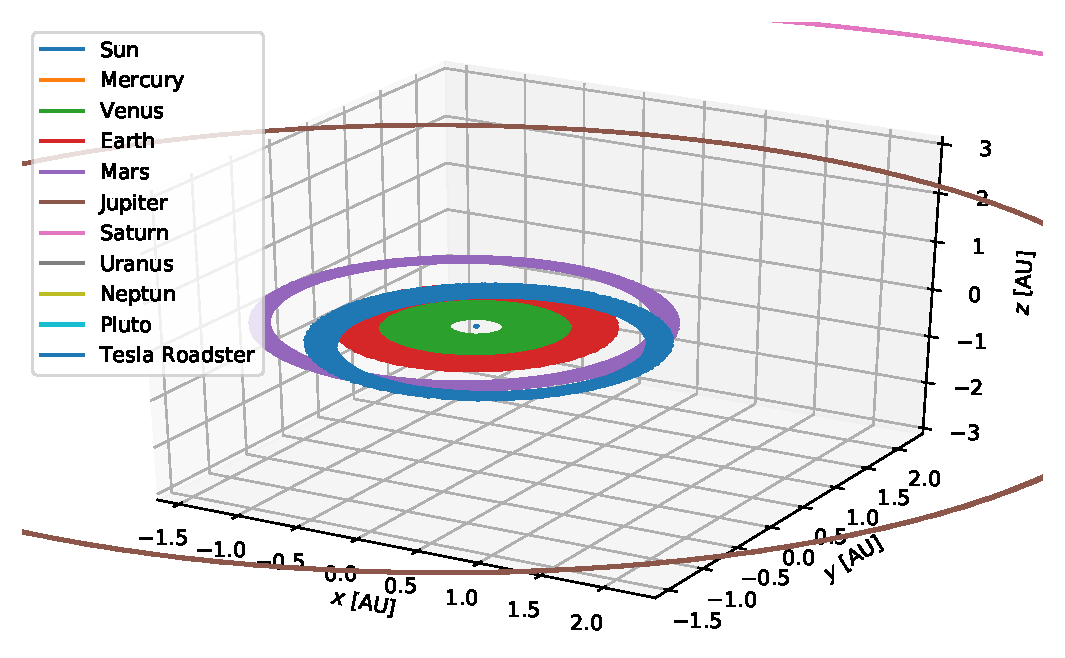
\includegraphics[scale=1]{Figures/InnerSolarSystem.pdf}
\caption{Zoom-in of full solar system}
\label{fig:outer}
\end{figure*}

\section{Discussion} \label{sec:discussion}

\section{Conclusion} \label{sec:conclusion}

\nocite{jensen:2019}
\newpage
\bibliography{ref}
\bibliographystyle{aasjournal}
\end{document}

% End of file `sample62.tex'.
